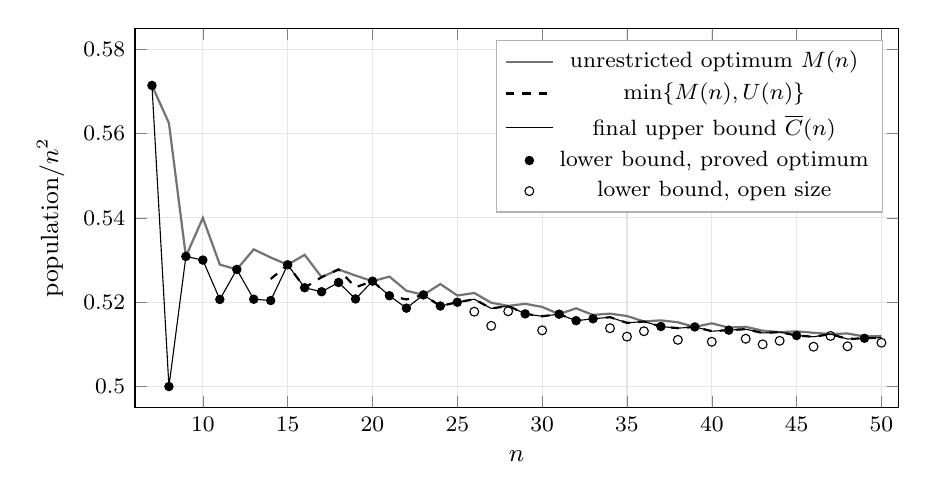
\begin{tikzpicture}
\begin{axis}[width=.93\textwidth,height=6.4cm,xlabel={$n$},ylabel={population$/n^2$},
 xmin=6,xmax=51,ymin=0.495,ymax=0.585,grid=both,grid style={black!10},
 legend style={font=\footnotesize,at={(0.98,0.97)},anchor=north east,draw=black!30},
 tick label style={font=\footnotesize},label style={font=\small}]
\addplot[black!55,thick,mark=none] coordinates {(7,0.57143) (8,0.56250) (9,0.53086) (10,0.54000) (11,0.52893) (12,0.52778) (13,0.53254) (14,0.53061) (15,0.52889) (16,0.53125) (17,0.52595) (18,0.52778) (19,0.52632) (20,0.52500) (21,0.52608) (22,0.52273) (23,0.52174) (24,0.52431) (25,0.52160) (26,0.52219) (27,0.51989) (28,0.51913) (29,0.51962) (30,0.51889) (31,0.51717) (32,0.51855) (33,0.51699) (34,0.51730) (35,0.51673) (36,0.51543) (37,0.51570) (38,0.51524) (39,0.51414) (40,0.51500) (41,0.51398) (42,0.51417) (43,0.51325) (44,0.51291) (45,0.51309) (46,0.51276) (47,0.51245) (48,0.51259) (49,0.51187) (50,0.51200)};
\addlegendentry{unrestricted optimum $M(n)$}
\addplot[black,thick,dashed,mark=none] coordinates {(14,0.52551) (15,0.52889) (16,0.52344) (17,0.52595) (18,0.52778) (19,0.52355) (20,0.52500) (21,0.52154) (22,0.52066) (23,0.52174) (24,0.51910) (25,0.52000) (26,0.52071) (27,0.51852) (28,0.51913) (29,0.51724) (30,0.51667) (31,0.51717) (32,0.51562) (33,0.51607) (34,0.51644) (35,0.51510) (36,0.51543) (37,0.51424) (38,0.51385) (39,0.51414) (40,0.51313) (41,0.51338) (42,0.51361) (43,0.51271) (44,0.51291) (45,0.51210) (46,0.51181) (47,0.51245) (48,0.51128) (49,0.51145) (50,0.51160)};
\addlegendentry{$\min\{M(n),U(n)\}$}
\addplot[black,thin,mark=none] coordinates {(7,0.57143) (8,0.50000) (9,0.53086) (10,0.53000) (11,0.52066) (12,0.52778) (13,0.52071) (14,0.52041) (15,0.52889) (16,0.52344) (17,0.52249) (18,0.52469) (19,0.52078) (20,0.52500) (21,0.52154) (22,0.51860) (23,0.52174) (24,0.51910) (25,0.52000) (26,0.52071) (27,0.51852) (28,0.51913) (29,0.51724) (30,0.51667) (31,0.51717) (32,0.51562) (33,0.51607) (34,0.51644) (35,0.51510) (36,0.51543) (37,0.51424) (38,0.51385) (39,0.51414) (40,0.51313) (41,0.51338) (42,0.51361) (43,0.51271) (44,0.51291) (45,0.51210) (46,0.51181) (47,0.51245) (48,0.51128) (49,0.51145) (50,0.51160)};
\addlegendentry{final upper bound $\overline C(n)$}
\addplot[only marks,mark=*,mark size=1.5pt,black] coordinates {(7,0.57143) (8,0.50000) (9,0.53086) (10,0.53000) (11,0.52066) (12,0.52778) (13,0.52071) (14,0.52041) (15,0.52889) (16,0.52344) (17,0.52249) (18,0.52469) (19,0.52078) (20,0.52500) (21,0.52154) (22,0.51860) (23,0.52174) (24,0.51910) (25,0.52000) (29,0.51724) (31,0.51717) (32,0.51562) (33,0.51607) (37,0.51424) (39,0.51414) (41,0.51338) (45,0.51210) (49,0.51145)};
\addlegendentry{lower bound, proved optimum}
\addplot[only marks,mark=o,mark size=1.6pt,black] coordinates {(26,0.51775) (27,0.51440) (28,0.51786) (30,0.51333) (34,0.51384) (35,0.51184) (36,0.51312) (38,0.51108) (40,0.51062) (42,0.51134) (43,0.51001) (44,0.51085) (46,0.50945) (47,0.51200) (48,0.50955) (50,0.51040)};
\addlegendentry{lower bound, open size}
\end{axis}
\end{tikzpicture}
